
\documentclass[10pt]{beamer}
\usepackage{kotex}

\usepackage{amsmath}
\usepackage{framed}
\usepackage{graphicx}
%https://www.overleaf.com/learn/latex/Inserting_Images

\usepackage{amsmath}
%use dfrac
\usepackage{xcolor}

\usepackage{amsthm}
%\usepackage{tabl}
\usepackage{listings}
\definecolor{mGreen}{rgb}{0,0.6,0}
\definecolor{mGray}{rgb}{0.5,0.5,0.5}
\definecolor{mPurple}{rgb}{0.58,0,0.82}
\definecolor{backgroundColour}{rgb}{0.95,0.95,0.92}
%https://tex.stackexchange.com/questions/348651/c-code-to-add-in-the-document
\lstdefinestyle{CppStyle}{
    backgroundcolor=\color{backgroundColour},   
    commentstyle=\color{mGreen},
    keywordstyle=\color{magenta},
    numberstyle=\tiny\color{mGray},
    stringstyle=\color{mPurple},
    basicstyle=\footnotesize,
    breakatwhitespace=false,         
    breaklines=true,                 
    captionpos=b,                    
    keepspaces=true,                 
    numbers=left,                    
    numbersep=5pt,                  
    showspaces=false,                
    showstringspaces=false,
    showtabs=false,                  
    tabsize=2,
    language=C++
}

\usepackage{url}

\usepackage{etoolbox}
\AtBeginEnvironment{quote}{\singlespacing\small}


\usepackage{thmtools}
\usepackage{xcolor}
\declaretheoremstyle[% spaceabove=6pt,spacebelow=6pt, headfont=\color{MainColorOne}\sffamily\bfseries, notefont=\mdseries, notebraces={[}{]}, bodyfont=\normalfont,
headpunct={},
postheadspace=1em,
%qed=▣,
]{maintheorem}

\declaretheorem[%
name=정의,
style=maintheorem,
numberwithin=section, shaded={%bgcolor=MainColorThree!20,
margin=.5em}]{dfn}
% \begin{dfn}[]
% \end{dfn}

\setbeamertemplate{footline}[frame number]

\usetheme{Hannover}
%\usetheme{CambridgeUS}


\title{시간복잡도 기초}

\author{EUnS}

\begin{document}


\begin{frame}{}
    \maketitle
\end{frame}    

% \begin{frame}{}
%     \tableofcontents
% \end{frame}   

\begin{frame}{$O, \Omega, \Theta$}
    \begin{itemize}
        \item $O(g(n)) = \{ f(n)$ 모든 $n \ge n_0$에 대해 $0 \le f(n) \le cg(n)$ 인 양의 상수 $c, n_0$이 존재한다. $\}$
        \pause
        \item $\Omega(g(n)) = \{ f(n)$ 모든 $n \ge n_0$에 대해 $0 \le  cg(n) \le f(n)$ 인 양의 상수 $c, n_0$이 존재한다. $\}$
        \pause
        \item $\Theta(g(n)) = \{ f(n)$ 모든 $n \ge n_0$에 대해 $0 \le  c_1 g(n) \le f(n) \le c_2g(n)$ 인 양의 상수 $c_1, c_2, n_0$이 존재한다. $\}$
    \end{itemize}
\end{frame}


\begin{frame}{그래프 모형}
    \begin{figure}[h!]
        \centering
        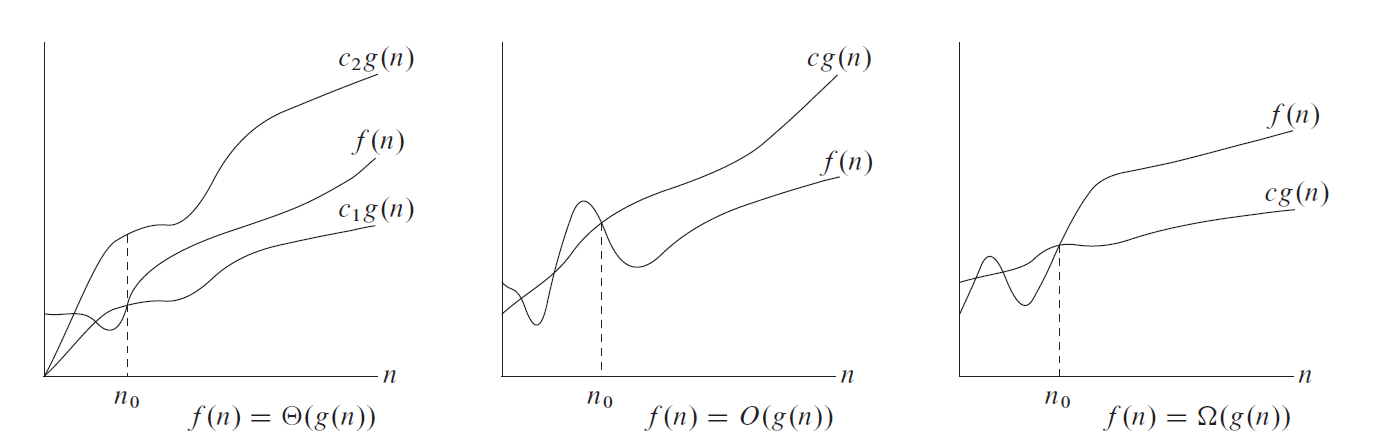
\includegraphics[scale=0.3]{pic1.PNG}
    \end{figure}
\end{frame}    



\begin{frame}{ex}
    \begin{itemize}
        \item $f(n) = n^2 + n + 3$
        \pause
        \item $O(2^n)$
        \pause
        \item $O(n^3)$
        \pause
        \item $O(n^2)$
        \pause
        \item $\Omega(1)$
        \pause
        \item $\Omega(n)$
        \pause
        \item $\Omega(n^2)$
        \pause
        \item $\Theta(n^2)$
    \end{itemize}
\end{frame}    

\begin{frame}{}
    \begin{itemize}
        \item $n_0$와 $c$는 내 마음대로 잡는다.
        \pause
        \item 극한에서 함수의 대소관계로 생각하면 제일 편함!
    \end{itemize}
\end{frame}    


\subsection{조화 급수의 상한과 하한}


\begin{frame}{조화 급수의 상한과 하한}
    $f(x) = \sum_{k=1}^n \dfrac{1}{k}$
    \pause
    \[
        \begin{aligned}
        \sum_{k=1}^n \dfrac{1}{k} 
        &\le \sum_{i=0}^{\lg n} \sum _{j=0}^{2^i-1} \dfrac{1}{2^i+j} \\ \pause
        &\le \sum_{i=0}^{\lg n} \sum _{j=0}^{2^i-1} \dfrac{1}{2^i} \\  \pause
        &=\sum_{i=0}^{\lg n} 1 \\ \pause 
        &\le \lg(n) + 1
        \end{aligned}
    \]
    $\sum_{k=1}^{n} \dfrac{1}{k} = O(\lg n)$
\end{frame}


\begin{frame}{적분을 이용한 상한,하한}

    단조 증가 함수 $f(k)$에 대해서 다음이 성립한다.
    $$\int_{m-1}^{n}f(x)dx \le \sum_{k=m}^n f(k) \le \int_{m}^{n+1}f(x)dx$$
    
    \begin{figure}[h!]
        \centering
        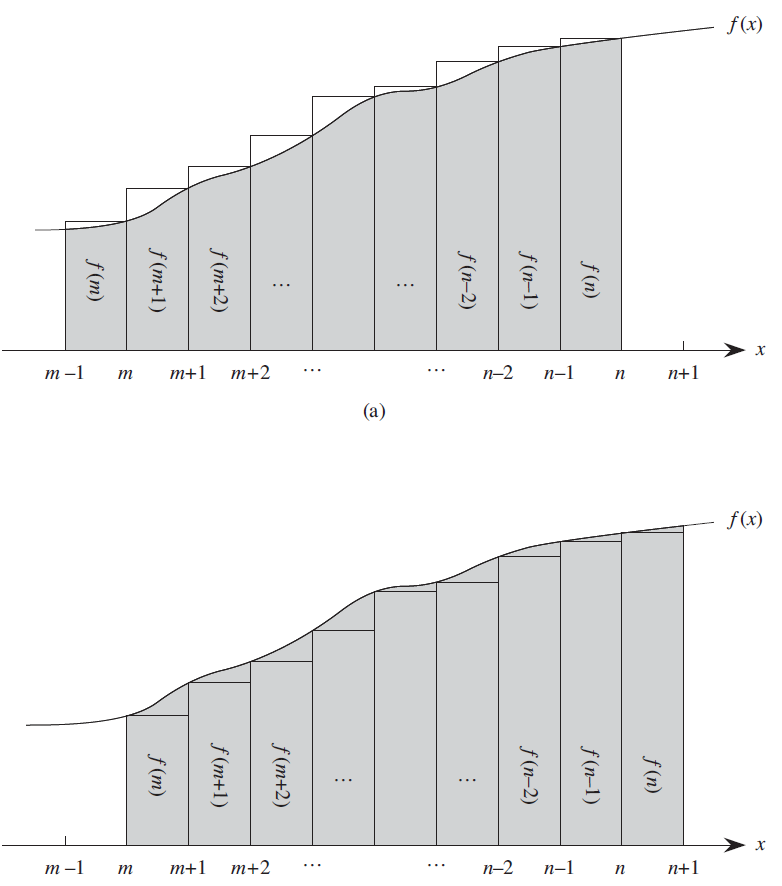
\includegraphics[scale=0.5]{./QuickSort/pic/q5.png}
        \caption{증가함수의 대소비교\cite{reference1}}
    \end{figure}
    
\end{frame}


\begin{frame}{적분을 이용한 상한,하한}

    단조 감소 함수 $f(k)$에 대해서 다음이 성립한다

    $$ \int_{m}^{n+1}f(x)dx \le \sum_{k=m}^n f(k) \le\int_{m-1}^{n}f(x)dx $$

\end{frame}




\begin{frame}{}
$    
\begin{aligned}
        &\sum_{k=2}^n \dfrac{1}{k}+1 \ge \int_{2}^{n+1}f(x)dx +1= \ln (n)+1 = \Omega(\ln n) \\
        &\int_{1}^{n+1}f(x)dx =\ln (n+1) = O(\ln n) \ge \sum_{k=1}^n \dfrac{1}{k}  \\
        & \therefore  \sum_{k=1}^n \dfrac{1}{k} = \Theta(\lg n)
    \end{aligned}
$
\end{frame}






\begin{frame}{스털링 근사}

$\lg(n!)$
\pause
$
    \begin{aligned}
             \int_1^n \lg(k) dx +1 \le \sum_{k=2}^n \lg k + 1 \le \int_2^{n+1} \lg(k) dx +1\\ \pause
             n \lg(n) -n + 1 \le \lg(n!) \le (n+1)\lg(n+1) -(n+1) -(2\lg2 - 2) \\ \pause
            \therefore \lg(n!) = \Theta(n\lg n)
    \end{aligned}
$

\end{frame}




\end{document}



% \begin{frame}{}
%     \begin{figure}[h!]
%         %\centering
%         \includegraphics[scale=0.25]{}
%         \caption{}
%     \end{figure}
% \end{frame}    

% \begin{frame}{$O$}
%     \begin{itemize}
%         \item 
%         \item 
%         \item 
%     \end{itemize}
% \end{frame}


% \begin{frame}{}
%     \href{}{\textcolor{blue}{참고}}
% \end{frame}    




%%%%%%%%%%%%%%%%%%%%%%%%%%%%%%%%%%%%%%%%%%%%%%%%%%%%%%%%%%%%%%%%%%%%%%%%%%%%%%%%%%%%%%%%%%%%%%%%%%%%%%%%%%%%%%%%%%%%%%%%%%%%%%%%%%%%%%%%%%%%%%%%%%%%%%%%%%%%%%%%%%%%%%%%%%%%%%%%%%%%%%%%%%%%%%%%%%%%%%%%%%%%%%%
